\newpage
\section{Durchführung}
\label{sec:Durchführung}

\begin{figure}
  \centering
  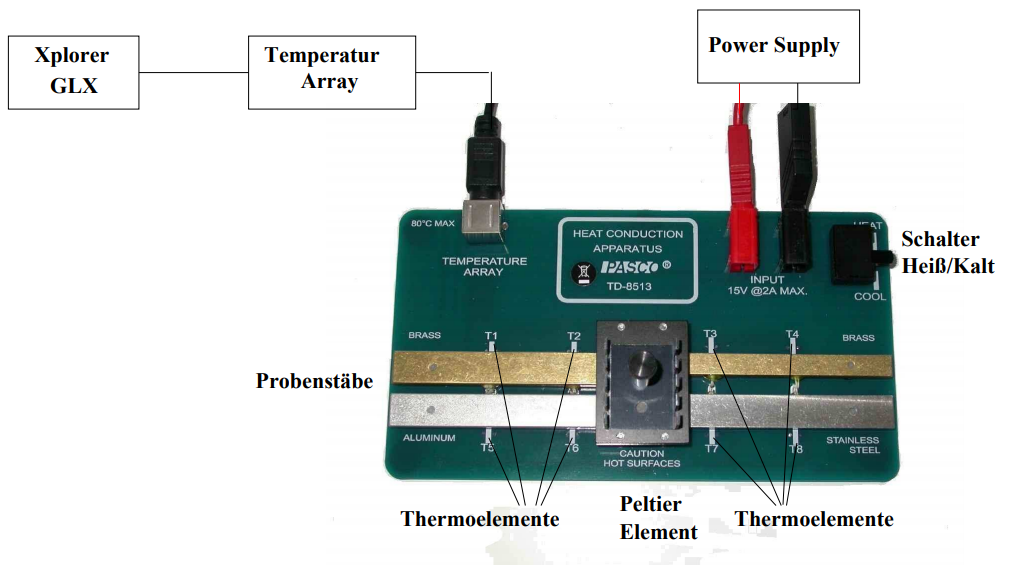
\includegraphics[width=0.98\textwidth]{content/aufbau.PNG}
  \caption{Veruschsaufbau ohne Isolierung.\cite[3]{v204}}
  \label{fig:aufbau}
\end{figure}

Das Versuchsaufbau ist in \autoref{fig:aufbau} zu sehen. Es befinden sich vier rechteckige Stäbe auf einer Grundplatte.
Diese bestehen aus Edelstahl, Aluminium und Messing. Es gibt zwei Messingstäbe, wovon einer eine größere Querschnittsfläche hat. 
Mittels eines Peltier-Elements werden diese Stäbe zeitgleich geheizt beziehungsweise gekühlt.
Besagtes Element wird an eine Spannungsquelle angeschlossen.

An je zwei Stellen an den Stäben werden die Temperaturen gemessen und mithilfe eines "Temperatur Arrays" an einen Datenlogger übertragen.
Mit diesem werden die Daten verechnet und grafisch dargestellt.

Während der Versuchsdurchführung liegt immer eine Isolation auf den Stäben, um den Wärmeaustausch mit der Luft zu minimieren.

Nach Abschluss jeder einzelnen Messreihe werden die Isolationen entfernt und die Stäbe auf mindestens 30°C heruntergekühlt.
Dazu wird der Schalter auf der Platte auf "COOL" gestellt.

Zunächst wird der Abstand zwischen den beiden Messstellen auf den Stäben gemessen.


\subsection{Die statische Methode}

Die Spannungszufuhr wird auf 5 V einstellt. Am Datenlogger wird eine Abtastrate von 5 s eingestellt und die Temperaturen an den acht Stellen als Funktion der Zeit gemessen.
Der Schlater auf der Platte wird auf "HEAT" gestellt.
Zunächst wird diese Messung 700 s lang durchgeführt.
Die gemessenen Werte werden als Funktion der Zeit grafisch dargestellt. Die Werte für T1, T4, T4 und T8 werden jeweils alle 140 s aufgenommen.

Mithilfe des Datenloggers werden die Temperaturdifferenzen von T7 und T8 sowie T2 und T1 als Funktion der Zeit geplottet.


\subsection{Die dynamische Variante - Angström-Messverfahren}

Die Spannungszufuhr wird auf 8 V eingestellt. Am Datenlogger wird die Abtastrate auf 2 s eingestellt und die Temperaturen werden an den acht Stellen gemessen.

In dieser Messreihe wird der Schalter periodisch von "HEAT" auf "COOL" beziehungsweise umgekehrt gestellt.

Für die  erste Messreihe beträgt die Periodendauer 80 s; der Schalter wird also alle 40 s umgeschaltet. Diese Reihe wird für die Dauer von zehn Perioden durchgeführt.
Die erhaltenen Daten von T1, T2 und T5, T6 werden aufgenommen und mithilfe des Datenloggers geplottet.

Die nächste Messreihe wird mit einer Periodendauer von 200 s durchgeführt. Es werden solange Daten aufgenommen, bis mindestens eines der Thermoelemente eine Temperatur von 80°C anzeigt. 
Die Temperaturverläufe von Edelstahl werden erneut mittels des Datenloggers grafisch dargestellt.